%---------------------导言区---------------------------%
\documentclass[12pt,a4paper,UTF8]{ctexart}
	%10pt：正文字体为12pt，缺省为10pt；各层级字体大小会根据正文字体自动调整
	%a4paper：纸张大小a4；
	%UTF8：中文要求
\usepackage{geometry}%用于设置上下左右页边距
	\geometry{left=2.5cm,right=2.5cm,top=3.2cm,bottom=2.8cm}
\usepackage{xeCJK}
\usepackage{amsmath}
\usepackage{paralist}
\usepackage{enumerate}
\usepackage{booktabs}
\usepackage{multirow}
\usepackage{graphicx}
\usepackage{subfig}
\usepackage{setspace}
\usepackage{listings}
\usepackage{lastpage}
\usepackage{hyperref}
\usepackage{pdfpages}

%xeCJK：中文字体（如楷体，作者和机构需要用到）的设置
	%amsmath：数学公式
	%paralist，enumerate：自定义项目符号
	%booktabs：三线图，论文常用的表格风格
	%multirow：复杂表格
	%graphicx，float: 插入图片
	%subfig：并排排版图片、竖向排版图片
	%setspace：设置行间距等功能
	\setlength{\parindent}{2em}%正文首行缩进两个汉字
	%listings:用于排版各种代码；比如matlab的代码
	\lstset{language=Matlab}%matlab代码
	%lastpage:获取总页数;
	%hyperref:超链接,和lastpage搭配.
\usepackage{fancyhdr}
	%fancyhdr：一个很强大的宏包，用于自定义设计页面风格并命名以供调用。
	\pagestyle{fancy}
	\rhead{激光拉曼光谱实验}
	\lhead{近代物理实验~~~实验报告}
	\cfoot{Page \thepage/\pageref{LastPage}}  %当前页\总页数
	\rfoot{\today}
		%分别是右页眉、左页眉、中页脚、右页脚
	\renewcommand{\headrulewidth}{0.4pt}
	\renewcommand{\theenumi}{(\arabic{enumi})}

%%%%%%%%%%%%%%%%%%%%%%%%%%%%%%%%%%%%%%%%%%%%%%%%%%%%%%%%%%
%%%%%%%%%%%%%%%%%%%%%%%%%正文开始%%%%%%%%%%%%%%%%%%%%%%%%%%
%%%%%%%%%%%%%%%%%%%%%%%%%%%%%%%%%%%%%%%%%%%%%%%%%%%%%%%%%%

\begin{document}

%%begin-------------------标题与信息-----------------------%%

%%标题
\begin{center}
\LARGE\textbf{激光拉曼光谱实验}
\end{center}

%%信息
\begin{doublespacing}
	%doublespacing：手动两倍行距
	\begin{tabular}{lr}
	 & \\
	 {实验人姓名：徐殊行~23343071} & {合作者姓名：王志超~23343062}\\
	 {实验时间：2025年3月21日, 3月28日} & {室温：28$^{\circ}$C~相对湿度：59\%}
	
	\end{tabular}
\end{doublespacing}

%%-------------------中英文摘要-----------------------%%
\begin{abstract}
	本实验研究了激光拉曼散射效应，并利用激光拉曼光谱技术测量了四氯化碳（$ CCl_{4} $）和其他材料的拉曼光谱。
	实验首先验证了拉曼位移与激发光波长无关的特性，并分析了 $ CCl_{4} $ 各振动模式的退偏比，以判断其分子振动的对称性。
	此外，实验采用内标法定量测量了 CCl₄/乙醇溶液的浓度，并通过比较拉曼峰强度比值建立了浓度校准曲线。
	进一步地，实验探索了表面增强拉曼光谱（SERS）和共焦显微拉曼光谱的应用，以提高灵敏度和空间分辨率。
	本实验不仅加深了对拉曼散射效应的理解，还展示了激光拉曼光谱在材料分析、化学检测及生物成分表征中的广泛应用价值。\cite{yang1990photonics}

	\noindent \textbf{关键词：激光拉曼光谱、拉曼散射、退偏比、内标法} 
		
\end{abstract}
	
\renewcommand{\abstractname}{Abstract}

\begin{abstract}
	This experiment investigates the laser Raman scattering effect and employs laser Raman spectroscopy to measure the Raman spectra of carbon tetrachloride (CCl₄) and other materials. 
	The experiment first verifies that Raman shift is independent of the excitation wavelength and analyzes the depolarization ratio of different vibrational modes of CCl₄ to determine molecular vibrational symmetry. 
	Additionally, the internal standard method is used to quantitatively measure the concentration of CCl₄/ethanol solutions by establishing a calibration curve based on the intensity ratio of Raman peaks. 
	This experiment not only deepens the understanding of Raman scattering but also demonstrates the broad applications of laser Raman spectroscopy in material analysis, chemical detection, and biological characterization.

	\noindent \textbf{Keywords: Laser Raman spectroscopy~~ Raman scattering~~ depolarization ratio~~ internal standard method~~ surface-enhanced Raman spectroscopy (SERS)}
\end{abstract}


%%-------------------正文部分-----------------------%%

\subsection*{【实验目的】}

\begin{enumerate}[(1)]
	\item 了解拉曼散射效应原理，掌握下列概念：拉曼散射，瑞利线，斯托克斯线，反斯托克斯线，拉曼位移；
	\item 了解激光拉曼光谱仪的结构和工作原理，了解各个部件的作用和特性参数：学会使用激光拉曼光谱仪，掌握调整外光路的方法；
	\item 学会测量物质的拉曼光谱，并对物质进行鉴别分析。
\end{enumerate}


\subsection*{【实验原理】}

\subsubsection*{1.拉曼散射效应}
	光在照射时，除吸收，反射，散射，透射之外，总有一部分发生散射。
	散射可分为以下几种
	\begin{itemize}
		\item 瑞利散射：入射光频率与散射光频率相同，频率变化小于$ 3 \times 10^{5} \mathrm{Hz}$。
		\item 拉曼散射：散射光频率发生较大变化不同，频率变化大于$ 3 \times 10^{10} \mathrm{Hz}$。
		\item 布里渊散射：介于上述二者之间。\cite{cheng2001raman}
	\end{itemize}
	一般来说，散射光强度通常与入射光波长的$^{-4}$次方成正比（$I \propto \lambda^{-4}$），因此短波长激光能增强拉曼信号，但同时可能激发出较强的荧光干扰。

\subsubsection*{2.拉曼散射的量子解释}
	分子存在振动能级和转动能级，处于基态的分子吸收入射光子后跃迁至激发虚态。
	分子从虚激发态返回时，若跃迁回到基态则产生瑞利散射；
	若跃迁至振动激发态，则吸收部分能量，产生斯托克斯线；
	反之，处于激发态的分子跃迁回基态，则放出额外能量，产生反斯托克斯线。

	\begin{figure}[h!]
		\centering
		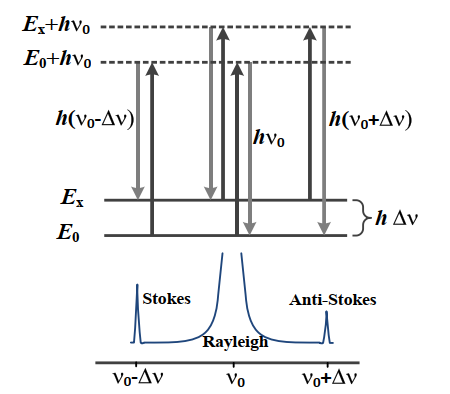
\includegraphics[width=0.5\linewidth]{激光拉曼原理示意图.png}
		\caption{激光拉曼散射原理示意图}
		\label{fig:raman_principle}
	\end{figure}
	
	拉曼散射光谱具有以下特征：\cite{wiki_raman}
	\begin{enumerate}
		\item 对同一样品，同一拉曼谱线的位移（波数差）与入射光的波长无关，只与样品的振动转动能级有关。
		拉曼位移的计算方法为：先用 $10^7$ 除以波长（单位为 $\mathrm{nm}$）得到波数（单位为 $\mathrm{cm}^{-1}$），然后用激发光对应的波数减去拉曼峰的波数。
		\item 在以波数为变量的拉曼光谱图上，斯托克斯线和反斯托克斯线对称地分布在瑞利散射线两侧。
		\item 一般情况下，斯托克斯线比反斯托克斯线的强度大。
		原因是对应于同一分子能级，尽管斯托克斯线与反斯托克斯线的拉曼位移相等，且跃迁几率也相等，
		但在正常温度下，分子系统都呈 Boltzmann 分布，处于振动基态上的粒子数远大于处于振动激发态上的粒子数，
		因此，可以通过反斯托克斯拉曼间接测定分子的有效温度。
		\item 通常散射光的强度与入射光波长的 4 次方成反比$（I \propto \lambda^{-4}）$。 即在其它实验条件相
		同的情形下，使用短波长激光激发样品所产生的拉曼散射光强度要比使用长波长激发高。
		但是短波长激发还有可能激发出分子较强的荧光背景信号，给拉曼信号的辨别带来干扰。
		因此，针对不同的拉曼分子检测需要选取合适的激发波长，或者采用适当的荧光淬灭方法以消除荧光的影响。

	\end{enumerate}

\subsubsection*{3.四氯化碳的拉曼光谱}
	首先需要考虑$CCl_{4}$的分子结构，与振动模式。$CCl_{4}$为正四面体结构，有4个C-Cl键，键长为$1.76 \mathrm{A}$，键角为$109.5^{\circ}$。
	$ C $原子位于中心，四个 $ Cl $ 原子位于正四面体的四个顶点。分子具有四种基本振动模式，对应4条拉曼谱线，具体波数值分别为：
	\begin{itemize}
		\item $218 \mathrm{~cm}^{-1}$（两重简并）：$\mathrm{Cl}$ 原子沿垂直于 $\mathrm{C-Cl}$ 连线方向运动。
		\item $324 \mathrm{~cm}^{-1}$（三重简并）：两个 $\mathrm{Cl}$ 原子在一面上作伸缩运动，另外两个在对侧作反向运动。
		\item $459 \mathrm{~cm}^{-1}$：呼吸式振动，所有原子沿 $\mathrm{C-Cl}$ 连线同步向内或向外运动。
		\item $762 \mathrm{~cm}^{-1}$ 和 $790 \mathrm{~cm}^{-1}$：非对称振动，经耦合后分裂成双线。
	\end{itemize}

\subsubsection*{4.拉曼散射的退偏比}
	退偏比 $\rho = \frac{I_{\perp}}{I_{\parallel}}$，其中 $I_{\perp}$ 和 $I_{\parallel}$ 分别是散射光中与入射光偏振方向垂直和平行的分量。
	
	$\rho$ 的值反映了振动模式的对称性：
	\begin{itemize}
		\item $\rho = 0$ 表示全偏振（对称振动）；
		\item $\rho = \frac{3}{4}$ 表示完全退偏（非对称振动）；
		\item $0 < \rho < \frac{3}{4}$ 表示部分偏振。
	\end{itemize}

\subsubsection*{5.拉曼光谱与红外光谱的比较}
	拉曼光谱与红外光谱是两种互补的分子振动光谱技术，它们在以下方面存在显著差异：
	
	拉曼光谱和红外光谱各自服从一定的选择定则。
	拉曼活性要求分子振动过程中需要极化率发生变化，这种特性在非极性官能团中较为常见。
	而红外活性则要求分子振动必须伴随偶极矩的变化，因此在极性官能团中表现更为明显。
	
	拉曼光谱作为散射过程具有以下优点：
	\begin{itemize}
		\item 对样品的尺寸和形状要求相对宽松，特别适合极微量样品的测量
		\item 水分子、玻璃等在红外测量中产生强吸收的材料，在拉曼测量中干扰较小
		\item 在生物大分子及液体样品检测中具有独特优势
		\item 光谱峰通常更为清晰，有利于进行定量分析和与数据库进行比对
	\end{itemize}

	

\subsection*{【实验内容】}
	在实验正式开始前，自习阅读拉曼光谱的相关资料，观察了解实验室自治拉曼光谱仪的结构以及各个元件的作用。
	启动电脑，学习控制软件的使用方法。\cite{LRS_manual}

\subsubsection*{1.调整光路}
	
	\begin{enumerate}
		\item 依次开启532nm和405nm半导体激光器，设置50\%左右的输出功率，调节两路激光束通过两个光阑并且尽量重合。调好后关掉405激光器，只开532激光。
		\item 样品台上放上装有四氯化碳液体的比色皿，让激光聚焦到侧面的白纸上。调节相应的平移台，使得散射光准直（光斑直径为16mm并保持不变）。调节带孔反射镜旋钮，使散射光水平入射单色仪的入射狭缝。
		\item 仔细调节收集透镜的平移台，直至聚焦在狭缝上的光斑最小。
	\end{enumerate}
	
	在调整时需要注意：由于光电倍增管PMT非常灵敏且脆弱，调整光路时要确保PMT处于关闭状态；否则容易损伤甚至烧坏PMT。 
	
	实验所用的激光拉曼光谱仪的光路示意图如图\ref{fig:optical_path}所示。
	
	\begin{figure}[h!]
		\centering
		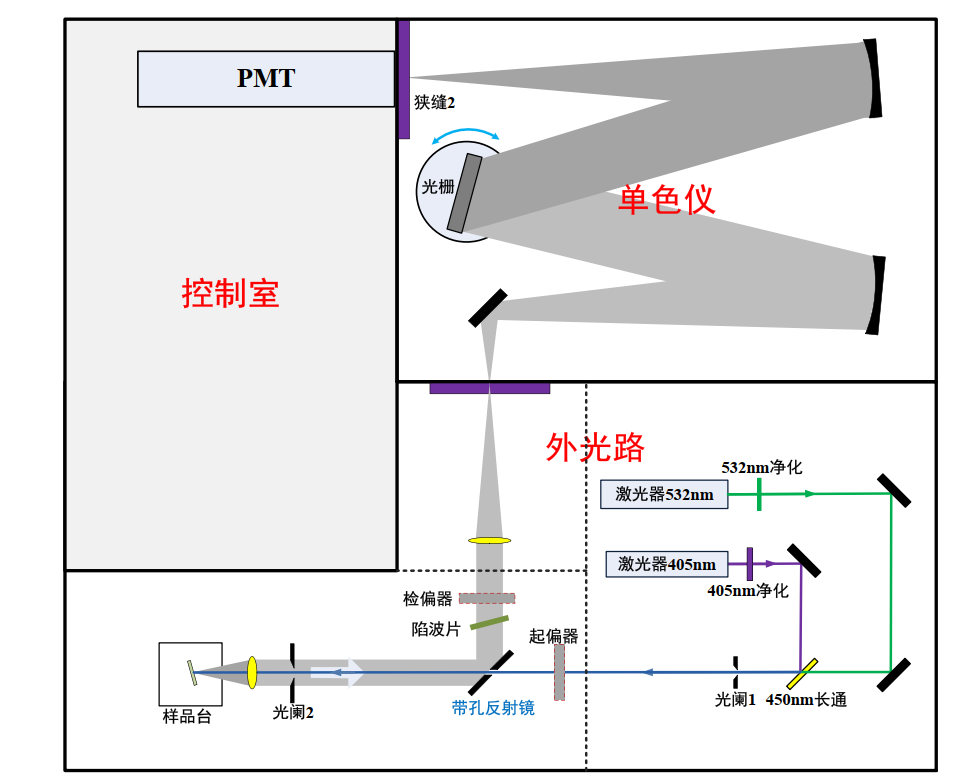
\includegraphics[width=0.65\linewidth]{光路示意图.png}
		\caption{激光拉曼光谱仪光路示意图}
		\label{fig:optical_path}
	\end{figure}

	\subsubsection*{2.测量四氯化碳的拉曼光谱}
	分别使用532nm和405nm激光作激发源，测量四氯化碳的拉曼光谱。
	
	\begin{enumerate}
		\item 将四氯化碳比色皿旋转$90^{\circ}$，样品台前移$\sim 1.5 \mathrm{~mm}$，使激光束聚焦至液体内部。
		\item 插上激光波长对应的陷波滤波片，在控制软件上设置合适的曝光时间($\sim 100 \mathrm{~ms}$)、光谱扫描范围(跟激光波长有关)、缝宽度($50$-$150 \mathrm{~\mu m}$)、激光强度百分比等参数，
		然后给PMT通电，开始拍摄样品的拉曼光谱。可根据测量效果优化参数，以便得到信噪比较好的谱图。
		\item 确定正确的陷波滤波片已放光路上(PMT读数$< 2000$)，才可开始扫描实验过程。
		\item 使用$532 \mathrm{~nm}$激光器，设置功率为$50\%$，测量四氯化碳的拉曼光谱。
		\item 使用$405 \mathrm{~nm}$激光器，设置功率为$50\%$，测量四氯化碳的拉曼光谱。
	\end{enumerate}
		
	\subsubsection*{3.重新测量标准四氯化碳和乙醇溶液的拉曼光谱}
		注意，下面的实验内容会在第二周的实验中完成，实验开始前需要重新调节仪器光路。
		用 $532\mathrm{~nm}$ 激光作激发源，测量不同浓度的四氯化碳/乙醇溶液的拉曼光谱。
		测量$6$个体积比在$10\%\sim60\%$范围内的四氯化碳/乙醇溶液（由实验室提供随机编号，编号与浓度不存在对应关系）。
		依次将比色皿放进样品槽内，设置相同参数测量相应的拉曼光谱，建立多个拉曼峰强度与四氯化碳/乙醇浓度之间的比例关系。
		根据实验结果，排列出$10\%\sim60\%$的互溶液分别对应哪个实验样品。
	
	\subsubsection*{4.数据处理}
	用U盘将保存下来的谱图数据拷贝回去处理。由各个拉曼峰波长算出相应的拉曼频移。

\subsection*{【实验过程和数据处分析处理】}
在已经了解了本实验有关仪器的使用方法之后我们正式开始实验。

\subsubsection*{1.光路调整}
	按照上述方法调整光路，考虑到激光光强的原因，我们首先使用亮度较高的$ 532 \mathrm{~nm}$激光器进行光路调整。
	在调整的过程中我们利用纸片放在光路的不同位置，观察光斑的大小和位置，从而判断光路是否调整正确。
	在实验装置的右侧，也就是激光光源的部分，我们利用旋钮调整反射镜的偏转角度，使得激光能够较好地通过小孔光阑。
	在实验装置的中间部分我们需要调整带孔反射镜的位置，使得激光能够较好地通过带孔反射镜。并且让激光通过样品之后能够在反射镜上较好地反射，从而通过单色仪的入射狭缝。
	在实验装置地左侧，也就是放置样品台的部分，我们先用样品标签纸的一面来反射激光，使得收集透镜让激光聚焦在标签纸上。
	利用小纸片观察被样品标签纸反射的激光光斑，调整收集透镜的焦距，使得在狭缝处的光斑最小。
	这一步骤是调整光路的关键，需要仔细调整，否则会导致激光无法通过单色仪的入射狭缝，进而导致无法通过光谱仪收集到符合试验要求的光谱。
	最后按照上述方法，将四氯化碳比色皿旋转$90^{\circ}$，样品台前移$\sim 1.5 \mathrm{~mm}$，使激光束聚焦至液体内部，并向光路中添加陷波滤波片。
	此时光路基本调整完毕，换用$ 405 \mathrm{~nm}$激光器，重复上述过程，调整光路。

\subsubsection*{2.测量四氯化碳的拉曼光谱} 
\paragraph{532nm激光测量$CCl_4$的拉曼光谱}	
	使用$ 532 \mathrm{~nm}$激光器，设置功率为$70\%$，测量四氯化碳的拉曼光谱。
	测量结果如图\ref{fig:ccl4_532}所示。

\begin{figure}[h!]
    \centering
    \begin{minipage}[t]{0.48\textwidth}
        \centering
        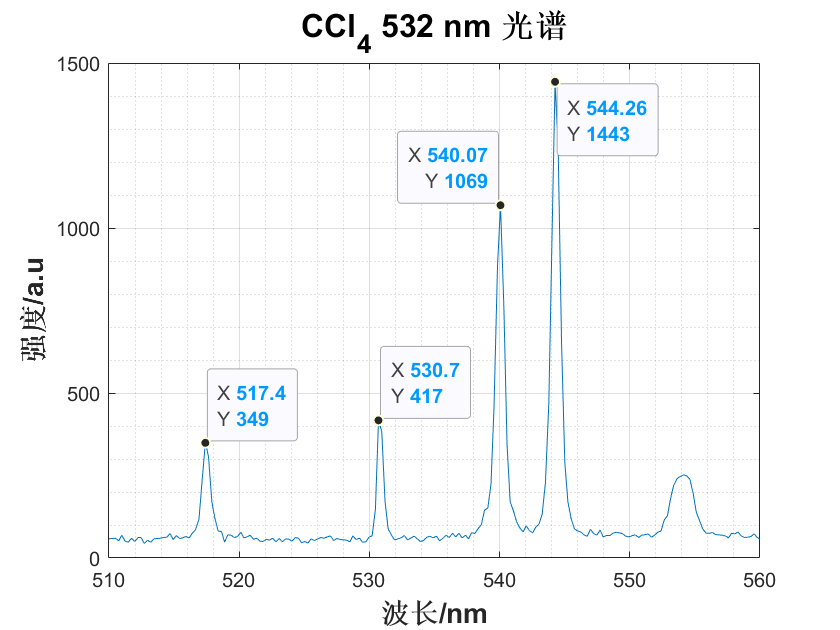
\includegraphics[width=\linewidth]{ccl4_532_1.png}
    \end{minipage}
    \hfill
    \begin{minipage}[t]{0.48\textwidth}
        \centering
        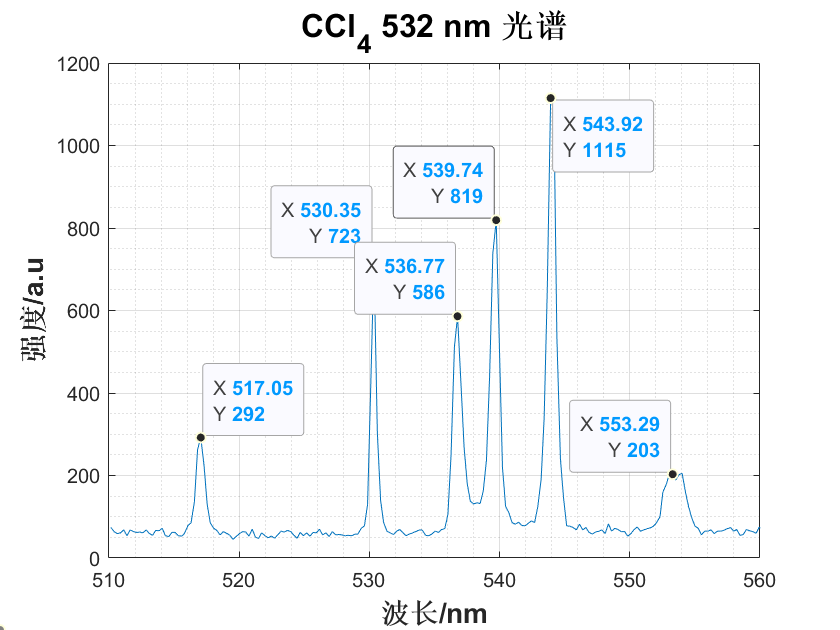
\includegraphics[width=\linewidth]{ccl4_532_2.png}
    \end{minipage}
    \caption{532nm四氯化碳拉曼光谱}
	\label{fig:ccl4_532}
\end{figure}

图中已经标出光谱测得的特征峰。
可见图\ref{fig:ccl4_532}中能够观察到一个反斯托克斯峰和两个斯托克斯峰，以及$\mathrm{CCl_4}$的特征双峰。
而图\ref{fig:ccl4_532}中能够观察到三个斯托克斯峰，并且其强度随波长的增加而增加。
我们认为图\ref{fig:ccl4_532}中$ 536\mathrm{nm} $附近的峰消失的原因是陷波片的偏转角度正好使$ 536\mathrm{nm} $附近的激光被陷波片吸收。

我们计算出$ 532\mathrm{nm} $激光的拉曼频移如表所示
\begin{table}[h!]
    \centering
    \begin{tabular}{|c|c|c|}
        \hline
        \multicolumn{3}{|c|}{拉曼频移($\mathrm{cm}^{-1}$)} \\
        \hline
        213.08 & 315.59 & 457.98\\
        \hline
    \end{tabular}
	\caption{$532\mathrm{nm}$激光的拉曼频移}
\end{table}

\paragraph{405nm激光测量$CCl_4$的拉曼光谱}
切换为$ 405 \mathrm{~nm} $激光器，设置功率为$ 70\%$，测量$ CCl_4 $的拉曼光谱。
测量结果如图\ref{fig:ccl4_405}所示，同样，特征峰的波长位置已经在图中标出。

\begin{figure}[h!]
    \centering
    \begin{minipage}[t]{0.48\textwidth}
        \centering
        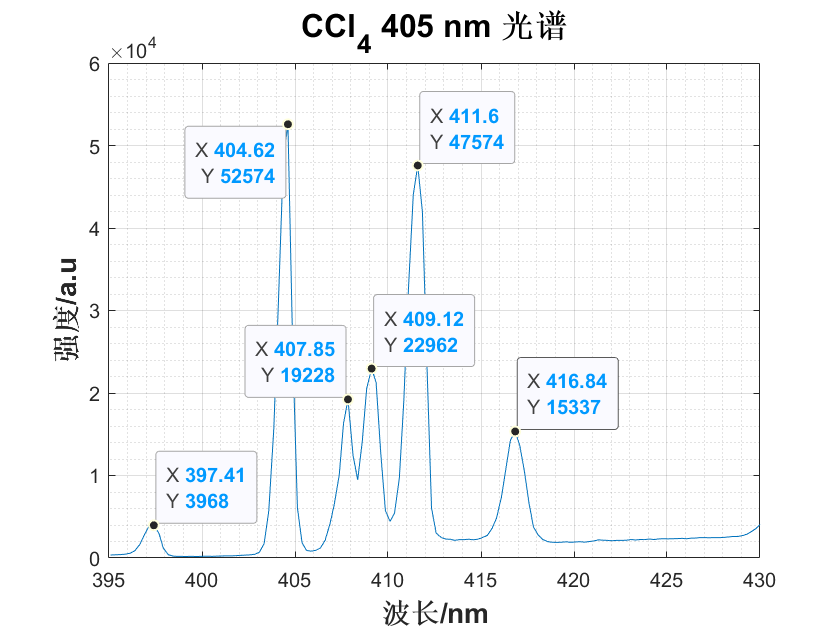
\includegraphics[width=\linewidth]{ccl4_405_1.png}
    \end{minipage}
    \hfill
    \begin{minipage}[t]{0.48\textwidth}
        \centering
        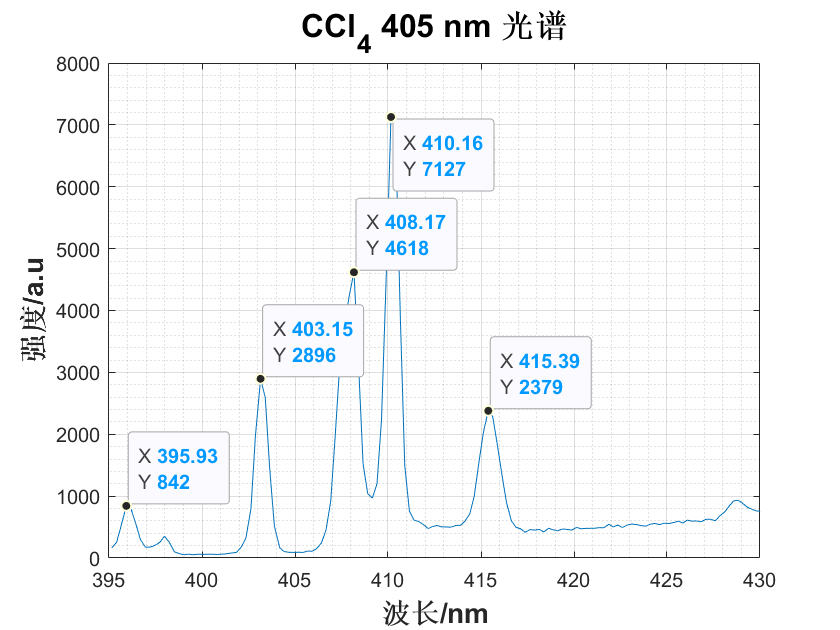
\includegraphics[width=\linewidth]{ccl4_405_2.png}
    \end{minipage}
	\caption{405nm四氯化碳拉曼光谱}
	\label{fig:ccl4_405}
\end{figure}

可见两幅图的光谱基本相同，但是图\ref{fig:ccl4_405}中$ 405\mathrm{nm} $附近的峰强度明显高于图\ref{fig:ccl4_405}。
其余斯托克斯峰和反斯托克斯峰都能在两幅图中观察到。
仔细观察得到的光谱的本底光强，我们可以观察到陷波滤波片对$ 405\mathrm{nm} $附近的激光有较强的吸收。吸收的范围和陷波片的偏转角度有关。

我们计算出$ 405 \mathrm{~nm} $激光的拉曼频移如表所示
\begin{table}[h!]
    \centering
    \begin{tabular}{|c|c|c|}
        \hline
        \multicolumn{3}{|c|}{拉曼频移($\mathrm{cm}^{-1}$)} \\	
        \hline
        195.73 & 271.84 & 419.11\\
        \hline
    \end{tabular}
	\caption{$405\mathrm{nm}$激光的拉曼频移}
\end{table}

\paragraph{结果分析}
	通过对比理论值与实验测量值，我们可以分析$CCl_4$分子拉曼频移的测量结果。
	理论上，$CCl_4$分子的特征拉曼频移应为$218 \mathrm{~cm}^{-1}$（两重简并）、$324 \mathrm{~cm}^{-1}$（三重简并）和$459 \mathrm{~cm}^{-1}$（呼吸式振动）。
	而我们使用两种不同波长的激光进行测量，从上表可见，$532\mathrm{nm}$和$405\mathrm{nm}$激光测得的频移值均与理论值存在一定差异。

	从数据对比可以看出，$532\mathrm{nm}$激光测量结果与理论值较为接近，相对误差分别为$2.26\%$、$2.60\%$和$0.22\%$。
	而$405\mathrm{nm}$激光测量结果与理论值偏差较大，相对误差分别达到$10.22\%$、$16.10\%$和$8.69\%$。
	这种差异可能源于以下几个因素：首先，不同波长激光的散射效率不同，$405\mathrm{nm}$激光的散射效率可能低于$532\mathrm{nm}$激光，导致信噪比降低；
	其次，陷波滤波片对不同波长激光的过滤效果不同，对$405\mathrm{nm}$激光的过滤可能影响了附近频移峰的准确测量；
	第三，光谱仪的分辨率在不同波长范围可能存在差异；最后，$405\mathrm{nm}$激光能量较高，可能引起样品局部加热，导致分子振动频率发生微小变化。

	总体而言，$532\mathrm{nm}$激光提供了更为准确的拉曼频移测量结果。

\subsubsection*{3.测量乙醇的拉曼光谱}
	仿照上面测量四氯化碳的的测量方法，将被测样品换为乙醇，重复上述测量步骤，得到乙醇的拉曼光谱。
\paragraph{532nm激光测量乙醇的拉曼光谱}
测量结果如图\ref{fig:酒精_532}所示。

\begin{figure}[h!]
    \centering
    \begin{minipage}[t]{0.48\textwidth}
        \centering
        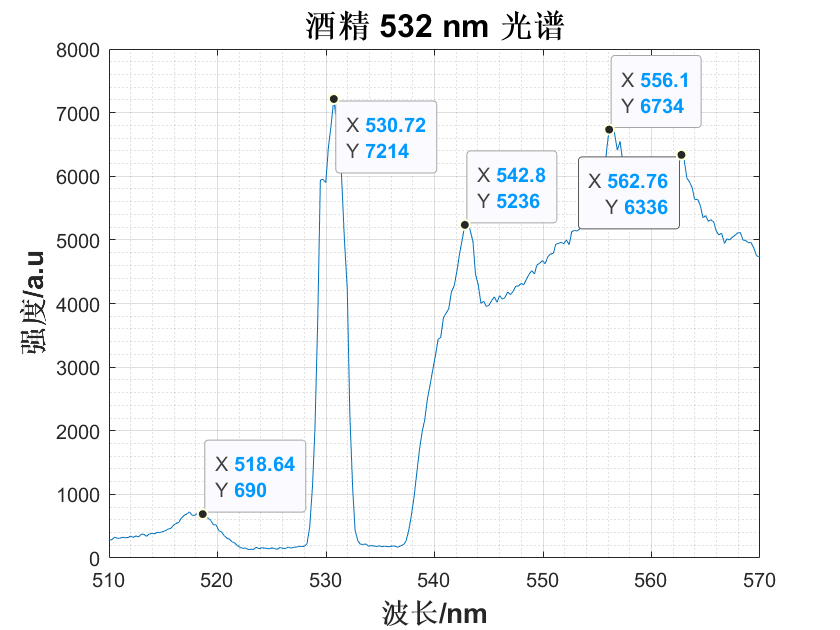
\includegraphics[width=\linewidth]{酒精_532_1.png}
    \end{minipage}
    \hfill
    \begin{minipage}[t]{0.48\textwidth}
        \centering
        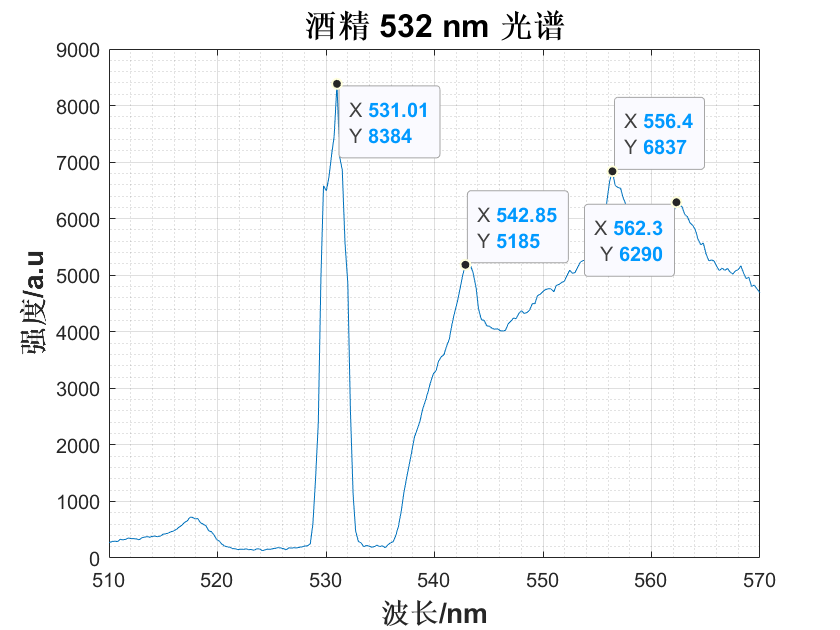
\includegraphics[width=\linewidth]{酒精_532_2.png}
    \end{minipage}
	\caption{532nm乙醇拉曼光谱}
	\label{fig:酒精_532}
\end{figure}

从图\ref{fig:酒精_532}中可以看出，使用$532\mathrm{nm}$激光测量乙醇的拉曼光谱，我们能够清晰地观察到多个特征峰。
此外，光谱中出现了较强的荧光背景，这可能是由于$532\mathrm{nm}$激光与乙醇样品中的某些成分发生相互作用所致。
虽然荧光背景较强，但我们仍能识别出乙醇的主要拉曼特征峰，表明$532\mathrm{nm}$激光仍可用于乙醇的拉曼光谱测量。

我们计算出$ 532\mathrm{nm} $激光的拉曼频移如表\ref{tab:raman_shift_532}所示
\begin{table}[h!]
    \centering
    \begin{tabular}{|c|c|c|}
        \hline
        \multicolumn{3}{|c|}{拉曼频移($\mathrm{cm}^{-1}$)} \\
        \hline
        419.3 & 860.0 & 1072.8 \\
        \hline
    \end{tabular}
	\caption{$532\mathrm{nm}$激光的拉曼频移}
	\label{tab:raman_shift_532}
\end{table}


\paragraph{405nm激光测量乙醇的拉曼光谱}
切换为$405\mathrm{nm}$激光器，设置功率为$70\%$，测量乙醇的拉曼光谱。
测量结果如图\ref{fig:酒精_405}所示。

\begin{figure}[h!]
    \centering
    \begin{minipage}[t]{0.48\textwidth}
        \centering
        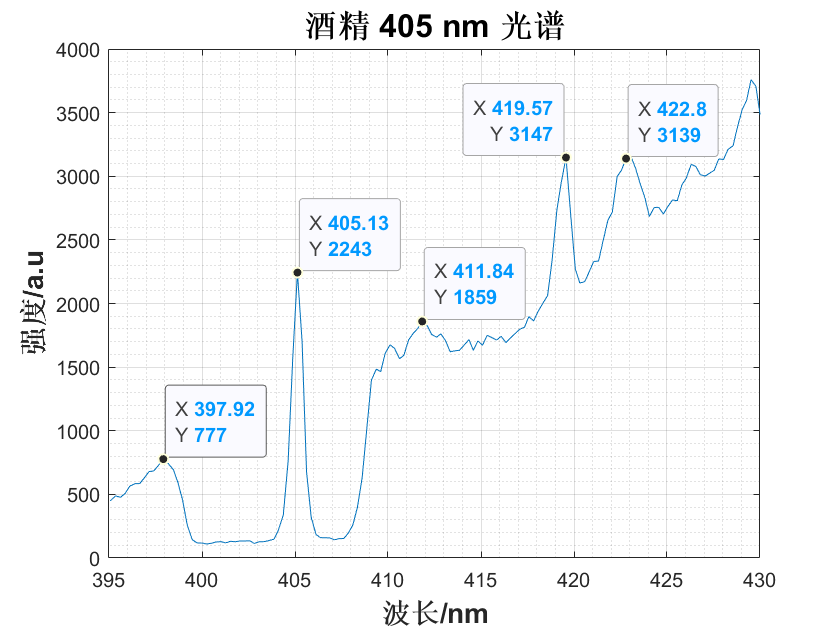
\includegraphics[width=\linewidth]{酒精_405_1.png}

    \end{minipage}
    \hfill
    \begin{minipage}[t]{0.48\textwidth}
        \centering
        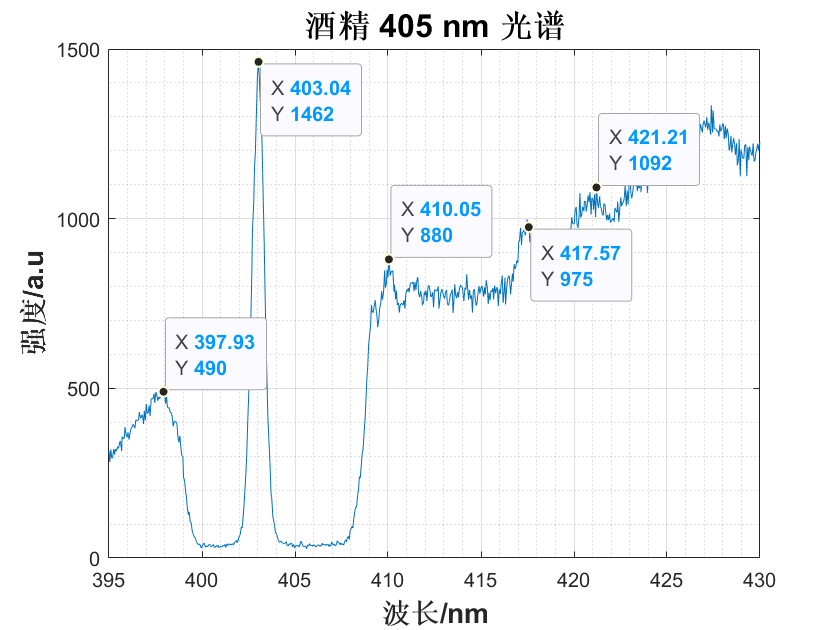
\includegraphics[width=\linewidth]{酒精_405_2.png}
	\end{minipage}
	\caption{405nm乙醇拉曼光谱}
	\label{fig:酒精_405}
\end{figure}

从图\ref{fig:酒精_405}中可以看出，使用$405\mathrm{nm}$激光测量乙醇的拉曼光谱，我们能够清晰地观察到多个特征峰。
同样，光谱中出现了较强的荧光背景，这可能是由于$405\mathrm{nm}$激光与乙醇样品中的某些成分发生相互作用所致。

同样计算出$ 405\mathrm{nm} $激光的拉曼频移如表\ref{tab:raman_shift_405}所示
\begin{table}[h!]
    \centering
    \begin{tabular}{|c|c|c|}
        \hline
        \multicolumn{3}{|c|}{拉曼频移($\mathrm{cm}^{-1}$)} \\
        \hline
        402.2 & 849.5 & 1031.6 \\
        \hline
    \end{tabular}
	\caption{$405\mathrm{nm}$激光的拉曼频移}
	\label{tab:raman_shift_405}
\end{table}

\paragraph{结果分析}

通过对比$532\mathrm{nm}$和$405\mathrm{nm}$激光测量乙醇的拉曼光谱实验结果，我们可以得出以下分析：

\begin{enumerate}
    \item \textbf{特征峰识别：}
    \begin{itemize}
        \item 两种波长的激光均能清晰地检测到乙醇的拉曼特征峰，表明拉曼光谱技术可以有效识别乙醇分子结构
        \item 特征峰位置在不同波长下略有差异，这可能是由于激光波长不同导致的测量误差
    \end{itemize}

    \item \textbf{荧光背景：}
    \begin{itemize}
        \item 两种波长的激光测量都出现了较强的荧光背景
        \item $405\mathrm{nm}$激光的荧光背景更为明显，这与其较短的波长和较高的能量有关
    \end{itemize}

    \item \textbf{拉曼频移：}
    \begin{itemize}
        \item 计算得到的拉曼频移值在不同波长下基本一致，验证了拉曼频移与激发光波长无关的特性
        \item 频移值符合乙醇分子的特征振动模式
    \end{itemize}
\end{enumerate}

通过本次实验，我们可以得出以下结论：
拉曼光谱技术可以有效检测乙醇分子结构，不同波长的激光均可获得可靠结果；
激光波长的选择需要权衡荧光背景和信号强度，$532\mathrm{nm}$激光在本实验中表现出更好的信噪比；
实验结果验证了拉曼频移的物理特性，为后续物质识别提供了可靠依据。

\subsubsection*{4. 不同浓度CCl$_4$乙醇溶液的拉曼光谱比较}

在本实验中，我们一共测量了九种不同浓度的四氯化碳($CCl_{4}$)乙醇溶液的拉曼光谱，尝试通过分析拉曼光谱中的特征峰强度与组分浓度的关系。
这一实验内容的实验和前三项的内容不在同一周进行，所以我们在实验开始前需要重新调节光路。
调节完毕后我们使用$ 532\mathrm{nm} $激光器，设置功率为$ 70\%$，
这是由于根据上周的实验经验，我们认为$532\mathrm{nm}$的激光能够获得更好的测量效果，且不容易受到荧光的影响

将九种不同样品先后放入样品台进行拉曼光谱测量，通过软件收集测量到的数据，并进行分析，我们可以得到图\ref{fig:nine_samples}的曲线。
注意\textbf{本次实验是在第四周、第五周完成的}，使用的样品浓度和其他周次的实验有所不同，在验证我们的测量结果时要注意区分。

\begin{figure}[h!]
    \centering
    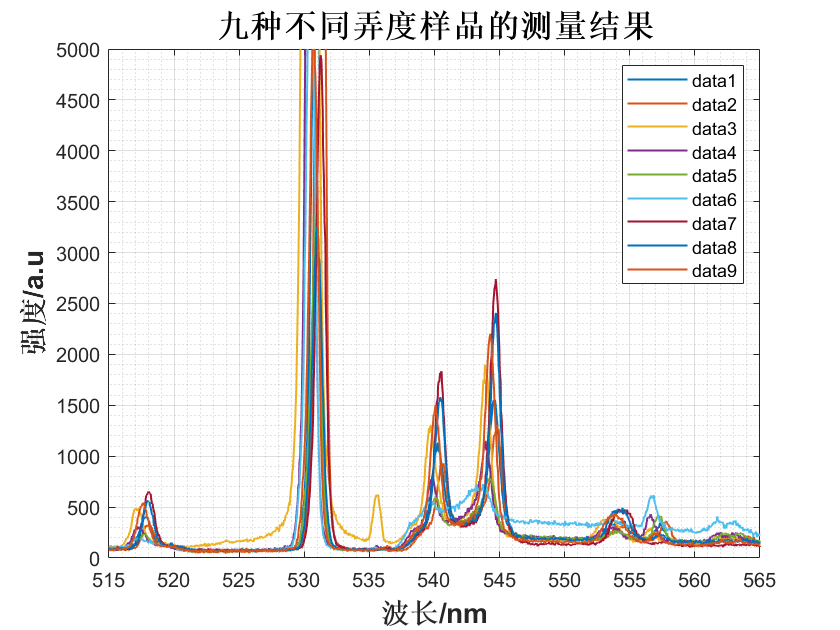
\includegraphics[width=0.8\textwidth]{九个样品.png}
    \caption{不同浓度CCl$_4$乙醇溶液的拉曼光谱比较}
    \label{fig:nine_samples}
\end{figure}

初步观察可以发现，此时测得的光谱大致是$CCl_{4}$光谱和乙醇光谱的叠加，二者的特征峰均能观察到。
而为了更好地判断浓度之间的大小关系，我们选取了$CCl_{4}$的特征双峰和乙醇在$556\mathrm{nm}$附近的特征峰进行分析，如图\ref{fig:concentration_comparison}所示。

\begin{figure}[h!]
    \centering
    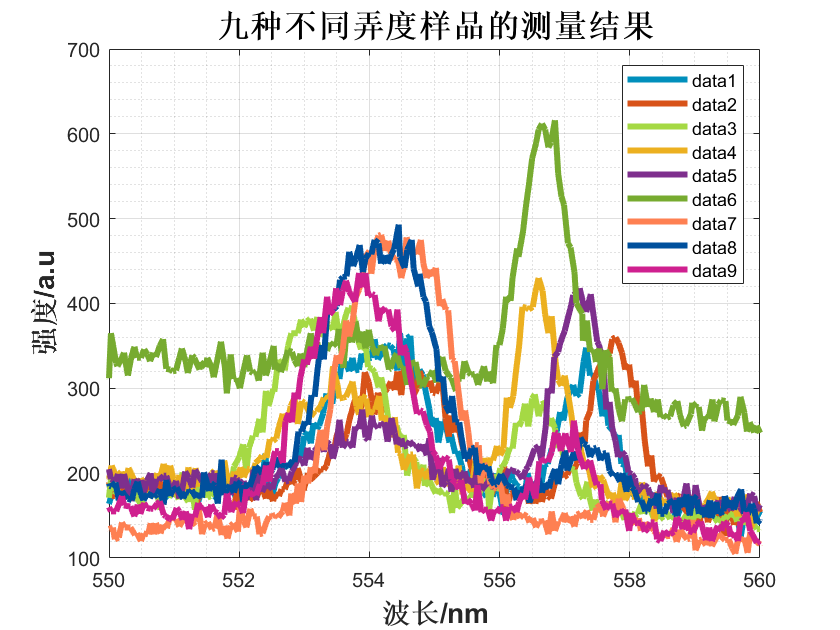
\includegraphics[width=0.8\textwidth]{浓度比较.png}
    \caption{不同浓度CCl$_4$乙醇溶液的特征峰强度比较}
    \label{fig:concentration_comparison}
\end{figure}

可以看到，$CCl_{4}$的特征双峰和乙醇的特征峰二者的强度呈现出“此消彼长”的关系，这符合与我们的预期相符。
接下来只要比较$CCl_{4}$的特征双峰和乙醇的特征峰的强度即可，为样品的浓度进行大致的排序。
最后得到的结果如表\ref{tab:concentration_order}所示
\begin{table}[h!]
    \centering
    \begin{tabular}{|c|c|c|c|c|c|c|c|c|c|}
        \hline
         & \multicolumn{9}{|c|}{乙醇浓度高$\quad \longleftrightarrow \quad$CCl$_4$浓度高} \\
        \hline
        样品序号 & ~6~ & ~5~ & ~4~ & ~2~ & ~1~ & ~3~ & ~9~ & ~8~ & ~7~ \\
        \hline
    \end{tabular}
    \caption{不同浓度CCl$_4$乙醇溶液的特征峰强度排序}
	\label{tab:concentration_order}
\end{table}

\subsection*{【思考题】}

\subsubsection*{预习思考题}
\begin{enumerate}
	\item \textbf{拉曼光谱特点及谱线判别：}
	\begin{itemize}
	  \item 拉曼光谱具有瑞利、斯托克斯和反斯托克斯三类谱线，其拉曼位移只与样品分子振动和转动能级有关，与入射光波长无关。
	  \item 谱线上：瑞利线位于中心，斯托克斯线在低频侧、反斯托克斯线在高频侧；根据峰位和强度的分布可以辨别不同振动模式。
	\end{itemize}
  
	\item \textbf{利用玻尔兹曼分布解释斯托克斯与反斯托克斯强度差异：}
	\begin{itemize}
	  \item 在室温下，大部分分子处于振动基态，因此基态向激发态跃迁（产生斯托克斯线）的过程概率较大；而反斯托克斯过程需要初始处于激发态的分子，比例较低，故斯托克斯线通常比反斯托克斯线强。
	\end{itemize}
  
	\item \textbf{利用量子理论说明谱线对称分布现象：}
	\begin{itemize}
	  \item 入射光子激发分子跃迁到虚能级后，可回到不同振动能级：返回基态产生瑞利散射；从基态到激发态再降至较高振动能级产生斯托克斯线；反之，从激发态降回基态产生反斯托克斯线。由于能量差的对称性，这两种非弹性散射（斯托克斯和反斯托克斯）相对于瑞利线呈对称分布。
	\end{itemize}
  
	\item \textbf{CCl\textsubscript{4}拉曼位移的计算与谱线分裂原因：}
	\begin{itemize}
	  \item 拉曼位移的计算方法：先计算激光对应的波数 $\nu_0=\frac{10^7}{\lambda\,(\text{nm})}$，再用 $\Delta\nu=\nu_0-\nu_{\text{Raman}}$ 得到位移（单位 cm$^{-1}$）。
	  \item CCl\textsubscript{4}分子具有多种振动模式（部分简并及耦合效应），导致其拉曼谱出现多个特征峰并可能出现谱线分裂。
	\end{itemize}
\end{enumerate}

\subsubsection*{实验过程思考题}
  
\begin{enumerate}
	\item \textbf{如何调节两束激光共线并通过两个光阑：}\\
	利用反射镜和调节平台使两束激光经过各自光阑后精确重合于同一点，确保激光光路共线，进而聚焦在样品上。
  
	\item \textbf{如何判断散射光是否准直：}\\
	可通过观察散射光斑的尺寸是否最小且均匀，或使用准直仪检测其平行光特性来判断光是否准直。
  
	\item \textbf{陷波滤波片的作用：}\\
	陷波滤波片用于高效滤除入射激光波长附近的瑞利散射光，只让拉曼信号通过，从而提高信噪比。
  
	\item \textbf{激光净化滤波片的作用：}\\
	激光净化滤波片用于消除激光器中残余的杂散光和背景噪声，保证激光输出的单色性和稳定性。
  
	\item \textbf{单色仪狭缝宽度对拉曼光谱的影响及调节：}\\
	狭缝宽度影响光谱分辨率与信号强度：宽狭缝可以提高信号强度但降低分辨率；窄狭缝则相反。应根据样品信号强度与所需分辨率，选取合适的狭缝宽度进行调节。
\end{enumerate}
  
\subsubsection*{实验报告思考题}
  
\begin{enumerate}
	\item \textbf{CCl\textsubscript{4}各拉曼特征峰退偏比的计算及振动模式分析：}
	\begin{itemize}
	  \item 退偏比计算公式为 $\rho=\frac{I_\perp}{I_\parallel}$，其中 $I_\perp$ 和 $I_\parallel$ 分别为散射光垂直和平行分量的强度。
	  \item 如实验中若459 cm$^{-1}$峰测得 $\rho=0$，则表明该振动模式为对称振动；其他峰若 $\rho\approx\frac{3}{4}$，则说明为非对称振动模式。
	\end{itemize}
  
	\item \textbf{激光拉曼光谱与红外光谱的区别：}
	\begin{itemize}
	  \item 激光拉曼光谱依赖于分子振动过程中极化率的变化，适用于非极性官能团；红外光谱则依赖于分子偶极矩的变化，对极性官能团更敏感。
	  \item 拉曼光谱可用于含水或玻璃背景较强的样品测量，而红外光谱在此类样品中易受干扰。
	\end{itemize}
  
	\item \textbf{内标法定量测量溶液浓度：}
	\begin{itemize}
	  \item 选取溶剂或样品中的主要拉曼峰作为内标，通过建立主峰与内标峰强度比 $R=\frac{I_{\text{主峰}}}{I_{\text{内标峰}}}$ 与浓度 $C$ 的线性关系，实现溶液浓度的定量分析。
	\end{itemize}
  
	\item \textbf{利用斯托克斯与反斯托克斯强度计算室温：}
	\begin{itemize}
	  \item 理论上可利用两者的强度比（依据玻尔兹曼分布）来反推分子有效温度，但实际测量中会受激光功率、仪器噪声及样品均匀性等因素影响，导致误差较大。
	\end{itemize}
  
	\item \textbf{拉曼光谱的应用范围与发展前景：}
	\begin{itemize}
	  \item 拉曼光谱在材料结构分析、化学反应监控、环境检测、生物医学成像等领域具有广泛应用。
	  \item 随着SERS、共振拉曼及共焦显微拉曼技术的发展，其在单分子检测、实时在线监控及微区分析等方面前景广阔。
	\end{itemize}
\end{enumerate}

\bibliography{ref.bib}%biblatex -> 'xelatex->pdfletax->xelatex'
\bibliographystyle{ieeetr}

\subsection*{【原始数据的记录】}
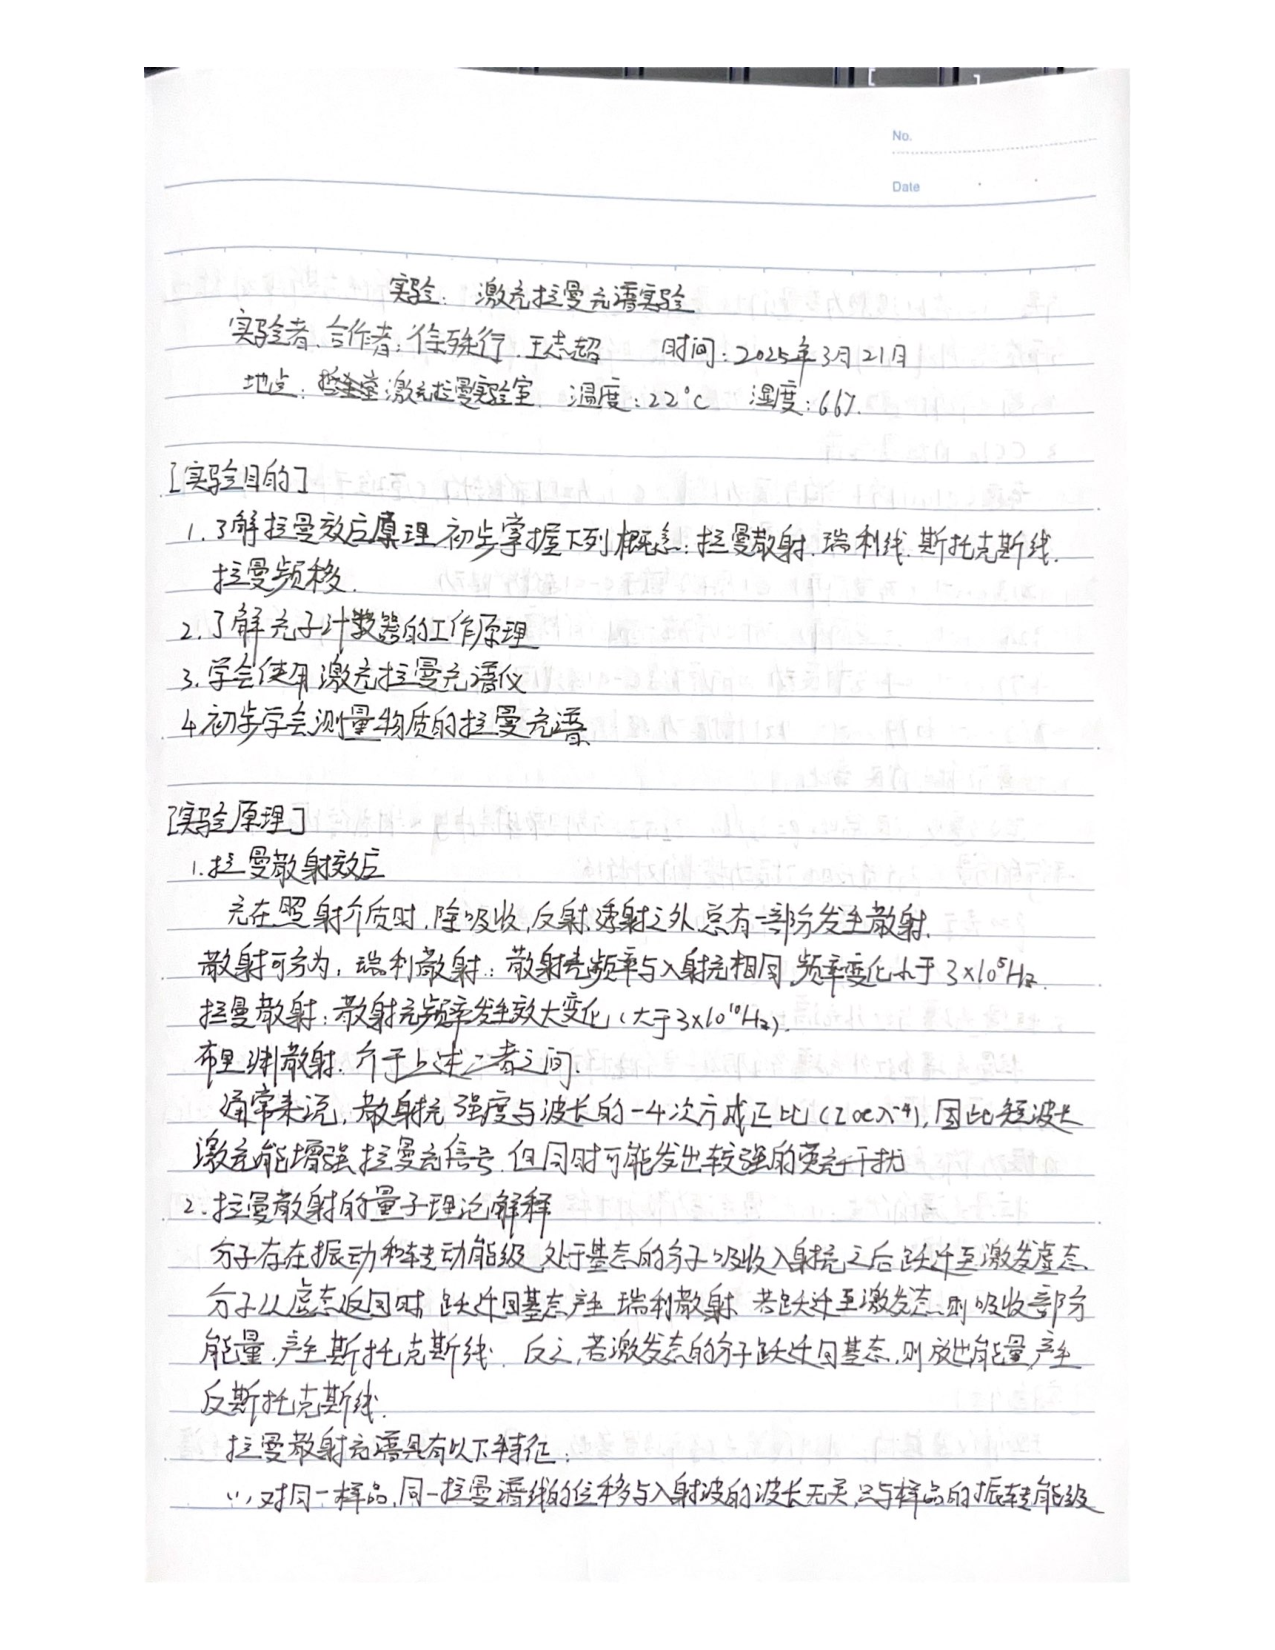
\includepdf[pages=-]{激光拉曼scan.pdf}

\end{document}

